\documentclass[10pt,a4paper]{article}
\usepackage[utf8]{inputenc}
\usepackage[english]{babel}
\usepackage{amsmath}
\usepackage{amsfonts}
\usepackage{amssymb}
\usepackage{graphicx}
\usepackage{subfigure}
\usepackage{nth}
\usepackage{wrapfig}
\usepackage[scale=0.8]{geometry}

\title{\vspace{-25mm}Reconsidering Generic Composition}
\author{Vincent Loup}
\date{May 29, 2017}

\begin{document}
\maketitle

\section{Introduction}
To create a secure communication channel, one should ensure the properties of confidentiality, authentication, and integrity.
For usability, cryptographers decided to look for simple encryption schemes that provide all those properties together.
These primitives are called authenticated encryption schemes (AE) and are widely used.
Currently, most used dedicated AE schemes are the GCM or CCM mode of operation \cite{dworkin2007sp}\cite{whiting2003counter}.
There also exists a competition called CAESAR that aims to identify new dedicated AE ciphers.
Here, we will only observe methods that have been devised to build an AE from a symmetric cipher and a MAC which was firstly analyzed by Bellare and Namprempre in 2000.
In 2014, Namprempre and Rogaway reconsidered the generic composition and obtained different results.

Given any MAC and any symmetric cipher, an AE scheme constructed with those primitives is considered secure if there does not exist an instance of a secure MAC and a secure cipher scheme that violate the properties of confidentiality, integrity, and authentication.

\section{Generic composition}
The first results from 2000 considered a probabilistic encryption scheme (pE) and a randomized MAC \cite{bellare2000authenticated}.
As a formalism, $E(K_e, M)$ is the encryption function that uses $K_e$ as the key and $M$ as the plaintext message that can be of variable length.
For the MAC scheme, the creation of the tag is done with $T(K_m, M)$ which is a function that takes the MAC secret key $K_m$ and the plaintext $M$.
The concatenation operation of two bit strings is written as $||$.
We build an AE scheme $\overline{E}(K_e||K_m, M)$ that has two symmetric keys and takes the plaintext $M$.
With those considerations, three possible constructions do exist.

\begin{itemize}
	\item Encrypt-and-MAC (E\&M): $\overline{E}(K_e||K_m, M) = E(K_e,M)||T(K_m, M)$.
		We compute the MAC of $M$ and concatenate it to the ciphertext.
		This method is used in the SSH protocol and we can compute $E(K_e,M)$ and $T(K_m, M)$ in parallel.
	\item MAC-then-Encrypt (MtE): $\overline{E}(K_e||K_m, M) = E(K_e,M||T(K_m, M))$.
		We devise the tag and concatenate it to the plaintext before encryption.
		It has the appearing advantage to encrypt the MAC, making it harder to attack.
		SSL is using this construction by default.
	\item Encrypt-then-MAC (EtM): $\overline{E}(K_e||K_m, M) = C||T(K_m,C)$ where $C = E(K_e, M)$.
		We encrypt the message and obtain $C$.
		Then, we compute the MAC of the ciphertext and we return the concatenation of $C$ with the tag.
		This method is used into the IPSec protocol.
\end{itemize}

The results from Bellare and Namprempre show that only the EtM construction is secure.
In the case of E\&M, the MAC is not required to provide confidentiality.
We can have a MAC scheme leaking part of the plaintext in its output.
Secondly, the MAC authenticates the plaintext and not the ciphertext.
It is broken if we have a malleable encryption scheme.
If we can find a second ciphertext such that it gets decrypted as the same plaintext, the MAC is identical.

For MtE, if an attacker finds a new ciphertext that decrypts to the same plaintext, the MAC is valid as well.

\section{Issue of the original approach}
So far, we considered a probabilistic encryption scheme and built a probabilistic authenticated-encryption scheme (pAE).
This approach does not apply with some real cryptographic algorithms since they are based on a nonce or an initialization vector (IV) that is provided externally.
Also, other AE schemes such as GCM, do provide the possibility to add some associated data (AD).
Associated data will only get authenticated, but not encrypted.
It is particularly good to use the associated data as information that is impossible to encrypt.
For example, for avoiding an attacker tampering or creating spoofed network packets, we may set the AD as the packet header since it can not be encrypted during transmission.

\section{Reconsidering generic composition}
Since we now need to include an IV or a nonce in those schemes, Namprempre and al revisited the problem of the generic composition in 2014 \cite{namprempre2014reconsidering}.
We define a nonce-based AE scheme (nAE) that takes a secret key $K$, a nonce $N$, the associated data $A$ and the plaintext $M$ to compute the ciphertext $C = E^{N,A}_K(M)$.
For decryption, we will compute $M = D^{N,A}_K(C)$.
The decryption algorithm is said to \emph{reject} if $D^{N,A}_K(C) = \bot$ and to \emph{accept} otherwise.
The properties of the nAE are as follows:
\begin{itemize}
	\item \emph{Correctness}: if $E^{N,A}_K(M) = C \not= \bot$ then $D^{N,A}_K(C) = M$.
	\item \emph{Tidiness}: if $D^{N,A}_K(C) = M \not= \bot$ then $E^{N,A}_K(M) = C$
\end{itemize}

Since we now have extra information to deal with (IV or nonce and AD) we need to redefine how a MAC is behaving.
Firstly, we introduce a vector-input MAC (or vecMAC).
This primitive is able to take one or more components as its input and output an authenticated tag.
It is useful to authenticate multiple values together in one step.
In our case, it will take 3 arguments that we may decide to provide or not.
Secondly, we have the classic string-input MAC (strMAC) which is the conventional MAC as we know it.
This primitive takes only one input to create the authenticated output tag.

For the encryption scheme, we may either use an IV-based encryption algorithm (ivE) or a nonce-based encryption algorithm (nE).
With an ivE, we need to set the IV as a random vector and for the nE, the nonce needs to be a unique initialization vector.

We will say that our nAE scheme is secure if it meets some security properties:
\begin{itemize}
\item The output of the encryption is indistinguishable from random strings in a chosen plaintext attack, to which the adversary must not repeat nonces.
\item No adversary is able to produce a valid ciphertext given an encryption oracle. Again, the adversary must not repeat nonces.
\end{itemize}

There exist many ways to build candidate schemes. 
We can start with a barebone model that has an encryption instance and one or two vecMAC instances.
Then, we can decide to connect the input or output of the different instances and parameters together to form a candidate scheme.
From this model, we can enumerate all candidates by listing the entire set of possible connections.
With a list of all candidates, it is possible to run a program that identifies attacks by finding security counterexamples.
With the remaining list of candidates without attacks, a manual analysis was done to prove the security of those schemes.

\subsection{AE from an ivE and a vecMAC}

\begin{figure}
\begin{center}
\begin{tabular}{ | c | c | c | }
	\hline
	Scheme & IV & Tag \\ \hline
	A1 & $F^{iv}_L(N,\sqcup,\sqcup)$ & $F^{tag}_L(N, A, M)$ \\ \hline
	A2 & $F^{iv}_L(N,A,\sqcup)$ & $F^{tag}_L(N, A, M)$ \\ \hline
	A3 & $F^{iv}_L(N,\sqcup,M)$ & $F^{tag}_L(N, A, M)$ \\ \hline
	A4 & $F^{iv}_L(N,A,M)$ & $F^{tag}_L(N, A, M)$ \\ \hline
	A5 & $F^{iv}_L(N,\sqcup,\sqcup)$ & $F^{tag}_L(N, A, C)$ \\ \hline
	A6 & $F^{iv}_L(N,A,\sqcup)$ & $F^{tag}_L(N, A, C)$ \\ \hline
	A7 & $F^{iv}_L(N,\sqcup,\sqcup)$ & $F^{tag}_L(N, A, M)$ \\ \hline
	A8 & $F^{iv}_L(N,A,\sqcup)$ & $F^{tag}_L(N, A, M)$ \\ \hline
	\hline
	A9 & $F^{iv}_L(N,A,\sqcup)$ & $F^{tag}_L(N, \sqcup, M)$ \\ \hline
	\hline
	A10 & $F^{iv}_L(N,A,\sqcup)$ & $F^{tag}_L(\sqcup, A, M)$ \\ \hline
	A11 & $F^{iv}_L(N,A,\sqcup)$ & $F^{tag}_L(\sqcup,\sqcup, M)$ \\ \hline
	A12 & $F^{iv}_L(N,\sqcup,\sqcup)$ & $F^{tag}_L(\sqcup, A, M)$ \\ \hline
\end{tabular}
\end{center}
	\caption{The twelve A schemes \cite{namprempre2014reconsidering}.\label{fig:aschemes}}
\end{figure}

To build a nAE from an ivE and a vecMAC, we chose a model that has two MAC instances and one encryption instance that is an ivE scheme.
One vecMAC $F^{iv}_L$ serves to create the random IV, while the other MAC $F^{tag}_L$ is creating the authenticated tag.
The MAC function takes three fixed arguments (nonce, associated data, plaintext or ciphertext) which we need to specify if we provide a value to this argument or not.
We denote the connection by explicitly writing the argument in its correct position.
When there is no connection in the MAC input, we will simply write $\sqcup$ as the argument.
The ivE scheme is just there to provide confidentiality and it may either take the plaintext message, or the concatenation of the plaintext with the tag.
We call candidates constructed in this way ``A schemes''.

Initially, there were 160 schemes to evaluate.
Only eight of them (A1 to A8) are \emph{favored} (they have a tight security bound), A9 is \emph{transitional} (it has a lower security bound), and three of them (A10 to A12) are \emph{elusive} (the authors were unable to prove its security, but no counterexample were found).
All twelves schemes are summarized in Figure \ref{fig:aschemes}.

\subsection{AE from an ivE and a strMAC}

\begin{figure}
	\centering 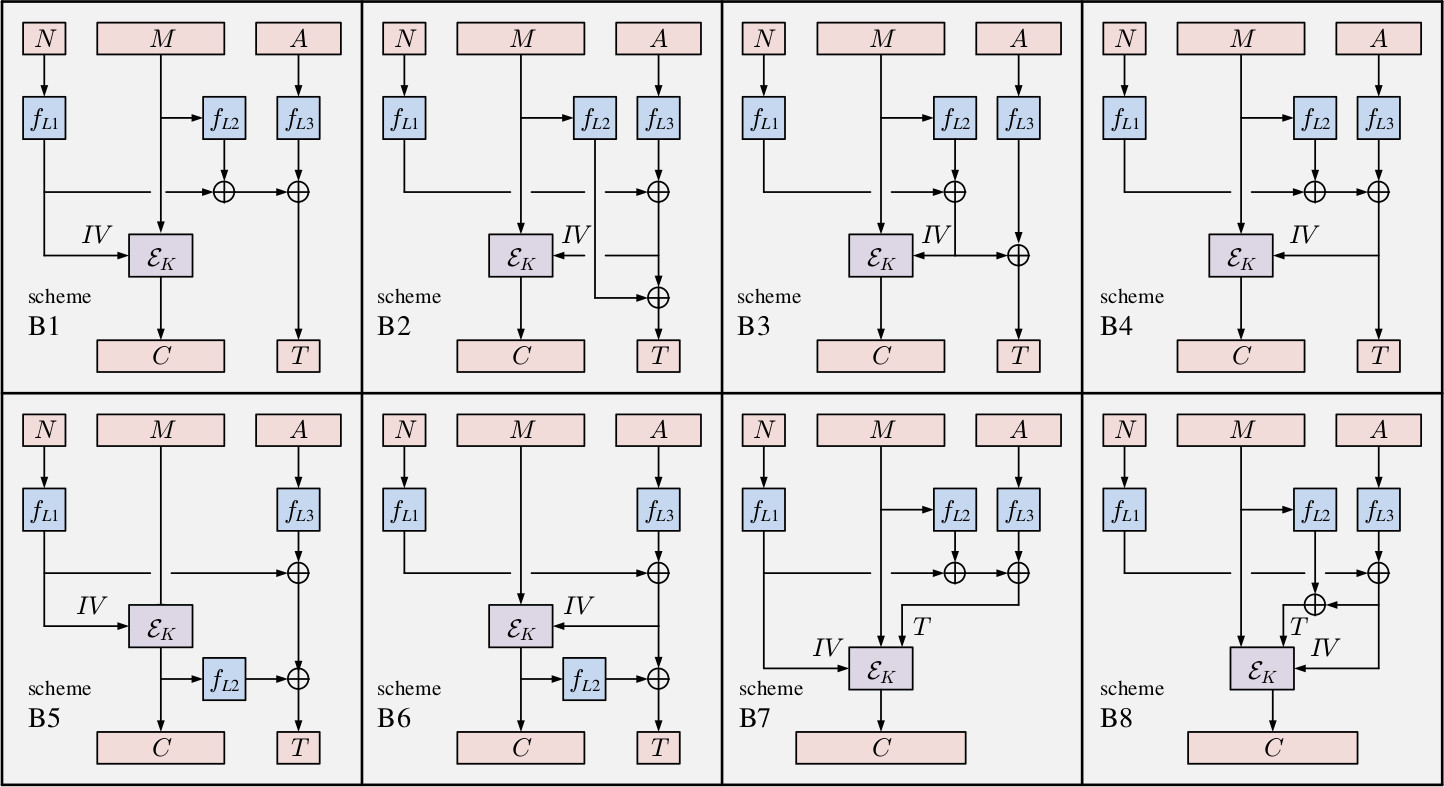
\includegraphics[scale=0.25]{strmac.jpg}
	\caption{The favored B schemes \cite{namprempre2014reconsidering}.\label{fig:bschemes}}
\end{figure}

The result of this modification gives us the eight ``B schemes'' as shown in Figure \ref{fig:bschemes}.
It is interesting to note that construction B1 is already known as the EAX construction.

A real MAC scheme is not like a vecMAC, but more like a strMAC.
For that matter, the authors presented the \emph{three-xor construction}.
It is an instanciation of a vecMAC using three strMAC that is proven secure.
We just compute each strMAC denoted as $f_L$ for each nonce, message and associated data to which we xor them together according to the vecMAC input.

\subsection{AE from an nE and a vecMAC}

\begin{figure}
	\centering 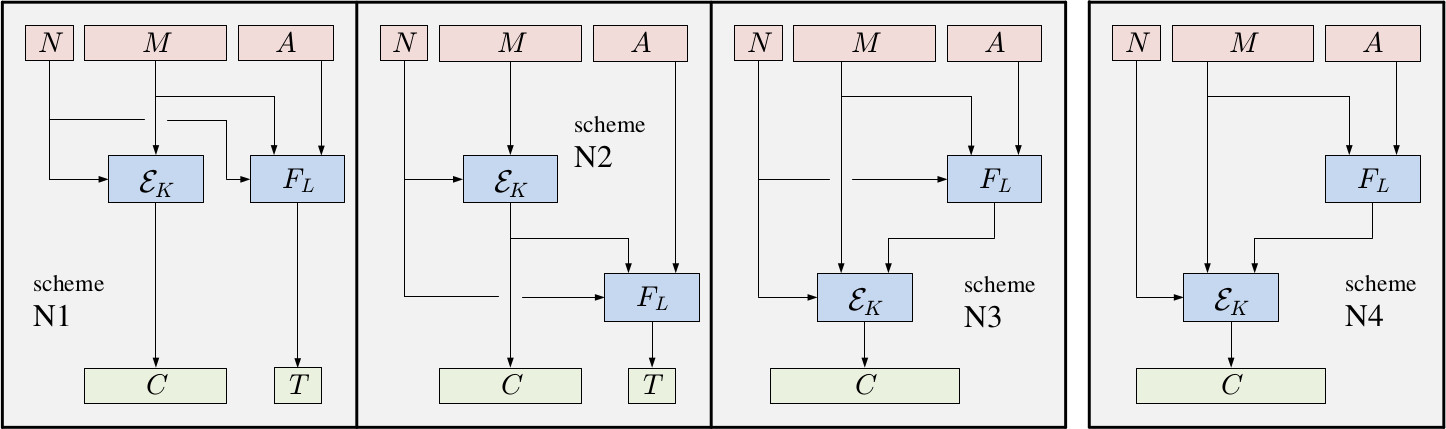
\includegraphics[scale=0.25]{noncemac.jpg}
	\caption{The favored N schemes \cite{namprempre2014reconsidering}.\label{fig:nschemes}}
\end{figure}

This time, we will construct an AE from a nonce-based encryption scheme and a vecMAC.
We will use the same method demonstrated earlier to select only the good schemes.

At first, there were only twenty candidates.
Out of these 20 candidates, only three were \emph{favored}, and one is \emph{elusive}.
We obtain the ``N schemes'' as shown in Figure \ref{fig:nschemes}.

\section{ISO-Standard for Generic Composition}
The ISO 19772 standard from 2009 explores the multiple approaches for having authenticated encryption \cite{iso197722009}.
It contains the classics of GCM, CCM or EAX but also the generic EtM construction.
On many points, the EtM standard is unsafe.

The standard defines a starting value (SV) which is unclear if it is a nonce or an IV from its definition.
Also, the SV is said to be communicated out of band and should be kept secret.
We do not know how to communicate it, hence how to prove its authenticity.
In the end, we do not know how to treat the SV, since it has not been covered in the results from Bellare and Namprempre in 2000.

Furthermore, no mentions are given about what to do if, during decryption, an error occurs because of some padding error.
There is also no mentions of possible associated data values.

In the end, it is not clear if this construction is a probabilistic AE or a nAE.
Other schemes covered in this documentation are described correctly.

\section{Conclusion}
In conclusion, both ISO standard and the two papers show that interpreting security results is not trivial since we may not be using the exact same schemes in the real world.
It also shows that additivity is never guaranteed, and that we should be careful on how to couple different schemes together since most of them do not work as we may expect.
We also have uncovered new secure schemes that are more concrete for being used with some real encryption and MAC schemes.

\begin{thebibliography}{9}

\bibitem{dworkin2007sp}
	Dworkin, Morris J,
	\emph{SP 800-38D. Recommendation for block cipher modes of operation: Galois/Counter Mode (GCM) and GMAC},
	National Institute of Standards \& Technology,
	2007

\bibitem{whiting2003counter}
	Whiting, Doug and Ferguson, Niels and Housley, Russell,
	\emph{RFC 3610. Counter with CBC-MAC (ccm)},
	2003

\bibitem{bellare2000authenticated}
	Bellare, Mihir and Namprempre, Chanathip,
	\emph{Authenticated encryption: Relations among notions and analysis of the generic composition paradigm},
	International Conference on the Theory and Application of Cryptology and Information Security,
	2000

\bibitem{namprempre2014reconsidering}
	Namprempre, Chanathip and Rogaway, Phillip and Shrimpton, Thomas
	\emph{Reconsidering generic composition},
	Annual International Conference on the Theory and Applications of Cryptographic Techniques,
	2014

\bibitem{ferguson2010cryptography}
	Ferguson, Niels and Schneier, Bruce and Kohno, Tadayoshi,
	\emph{Cryptography Engineering: Design Principles and Practical Applications},
	Wiley Publishing, Inc.,
	2010

\bibitem{iso197722009}
	ISO/IEC 19772,
	\emph{Information technology - Security techniques - Authenticated encryption},
	2009

\end{thebibliography}

\end{document}
